\documentclass[
    12pt,
    openright,
    oneside,
    a4paper,
    english,
    brazil,
    sumario=tradicional
]{abntex2}

% 1. Carrega as configurações e pacotes
\usepackage{lmodern}
\usepackage[T1]{fontenc}
\usepackage[utf8]{inputenc}

\usepackage{indentfirst}
\usepackage{microtype}
\usepackage{graphicx}
\usepackage{amsmath,amssymb}
\usepackage{booktabs}
\usepackage{longtable}
\usepackage{array}
\usepackage{multirow}
\usepackage{float}
\usepackage{caption}
\usepackage{subcaption}
\usepackage{xcolor}
\usepackage{url}
\usepackage{hyperref}

\usepackage[alf]{abntex2cite}
\usepackage{listings}

\definecolor{codebg}{RGB}{248,248,248}
\definecolor{codekw}{RGB}{0,102,204}
\definecolor{codecm}{RGB}{0,128,0}
\definecolor{codestr}{RGB}{163,21,21}

\lstdefinestyle{base}{
    backgroundcolor=\color{codebg},
    basicstyle=\ttfamily\footnotesize,
    breaklines=true,
    numbers=left,
    numberstyle=\tiny\color{gray},
    numbersep=8pt,
    frame=single,
    rulecolor=\color{gray!40},
    showstringspaces=false,
    tabsize=4,
    captionpos=b,
    escapeinside={(*@}{@*)} % <--- Isso resolve os avisos de caracteres especiais
}

\lstdefinestyle{cstyle}{
    style=base,
    language=C,
    commentstyle=\color{codecm}\itshape,
    keywordstyle=\color{codekw}\bfseries,
    stringstyle=\color{codestr}
}

\lstdefinestyle{x86}{
    style=base,
    language=[x86masm]Assembler,
    commentstyle=\color{codecm}\itshape,
    keywordstyle=\color{codekw}\bfseries
}

\lstdefinelanguage{ARMAssembly}{
    morekeywords={mov,add,sub,mul,ldr,str,ldp,stp,b,bl,ret,beq,bne,cbz,cbnz,cmp,adrp,adr,lsl,lsr,asr},
    sensitive=false,
    morecomment=[l]{//},
    morecomment=[s]{/*}{*/},
    morestring=[b]"
}

\lstdefinestyle{arm}{
    style=base,
    language=ARMAssembly,
    commentstyle=\color{codecm}\itshape,
    keywordstyle=\color{codekw}\bfseries,
    stringstyle=\color{codestr}
}

\lstdefinelanguage{RISCVAssembly}{
    morekeywords={lw,sw,add,sub,and,or,xor,beq,bne,blt,bge,jal,jalr,li,la,mv,ret,lui,auipc,slli,srli},
    sensitive=false,
    morecomment=[l]{\#},
    morestring=[b]"
}

\lstdefinestyle{riscv}{
    style=base,
    language=RISCVAssembly,
    commentstyle=\color{codecm}\itshape,
    keywordstyle=\color{codekw}\bfseries,
    stringstyle=\color{codestr}
}

\renewcommand{\lstlistingname}{Código}
\renewcommand{\lstlistlistingname}{Lista de códigos}
\renewcommand{\figurename}{Figura}
\renewcommand{\tablename}{Tabela}

\hypersetup{
    colorlinks=true,
    linkcolor=black,
    citecolor=black,
    urlcolor=blue,
    pdftitle={Funcionamento da memória cache e técnicas de otimização},
    pdfauthor={Arthur Martins Fonseca Dias; Arthur Freitas Araújo; Caio Seabra de Queiroz; Marina Souza Ramos}
}

\usepackage{titlesec}

\titleformat{\section}
{\normalfont\bfseries\raggedright}
{\thesection}
{1em}
{}

\titleformat{\subsection}
{\normalfont\bfseries\raggedright}
{\thesubsection}
{1em}
{}

\titleformat{\subsubsection}
{\normalfont\raggedright}
{\thesubsubsection}
{1em}
{}

\titlespacing*{\section}{0pt}{3.5ex plus 1ex minus .2ex}{2.3ex plus .2ex}
\titlespacing*{\subsection}{0pt}{3.25ex plus 1ex minus .2ex}{1.5ex plus .2ex}
\titlespacing*{\subsubsection}{0pt}{3.25ex plus 1ex minus .2ex}{1.5ex plus .2ex}

% ---------- Comandos personalizados para os dados do trabalho ----------
\providecommand{\curso}[1]{\def\imprimircurso{#1}}
\providecommand{\imprimircurso}{}
\providecommand{\disciplina}[1]{\def\imprimirdisciplina{#1}}
\providecommand{\imprimirdisciplina}{}
\providecommand{\professor}[1]{\def\imprimirprofessor{#1}}
\providecommand{\imprimirprofessor}{}

% 2. Define os dados do trabalho (isso vai preencher a capa automaticamente)
\titulo{Funcionamento da memória cache e técnicas de otimização}
\autor{Arthur Freitas Araújo \\ Arthur Martins Fonseca Dias \\ Caio Seabra de Queiroz \\ Marina Souza Ramos}
\local{Brasília -- DF}
\data{2026}
\instituicao{Universidade Católica de Brasília}
\curso{Ciência da Computação}
\disciplina{Arquitetura de Computadores}
\professor{Weldes Lima Oliveira}

\begin{document}

% --- Pré-textuais ---
\begin{capa}
    \centering

    % Instituição e Curso
    {\ABNTEXchapterfont\large\imprimirinstituicao\par}
    \vspace{0.5cm}
    {\ABNTEXchapterfont\large\imprimircurso\par}

    \vspace*{3cm}

    % Autores
    {\ABNTEXchapterfont\large\imprimirautor\par}

    \vspace*{2cm}

    % Título
    {\ABNTEXchapterfont\bfseries\Large\imprimirtitulo\par}

    \vfill

    % Texto de apresentação alinhado à direita
    \begin{flushright}
        \begin{minipage}{0.6\textwidth}
            \SingleSpacing
            Relatório técnico-acadêmico apresentado à \imprimirinstituicao, como parte dos requisitos avaliativos da unidade curricular de \imprimirdisciplina. \\
            Professor: \imprimirprofessor.
        \end{minipage}
    \end{flushright}

    \vfill

    % Local e Data
    {\large\imprimirlocal\par}
    {\large\imprimirdata\par}

\end{capa} % Apenas a capa unificada

\pdfbookmark[0]{\contentsname}{toc}
\tableofcontents*
\cleardoublepage

% --- Textuais (O Tema 1 em si) ---
\textual

\chapter{Introdução}
\label{cap:introducao}

\section{Contextualização}
A memória cache é uma memória volátil de alta velocidade, porém com pequena capacidade de armazenamento. O tempo de acesso a um dado nela contido é muito menor que se o mesmo estivesse na memória principal. O propósito do uso da memória cache é minimizar a disparidade existente entre a velocidade com que o processador executa instruções e a velocidade com que dados são lidos e gravados na memória principal. Apesar de ser uma memória de acesso rápido, a capacidade de armazenamento das memórias cache é limitada em função do seu alto custo.

A memória cache armazena uma pequena parte do conteúdo da memória principal. Toda vez que o processador faz referência a um dado armazenado na memória, é verificado, primeiramente, se o mesmo encontra-se na memória cache. Caso o processador encontre o dado (\textit{cache hit}), não há necessidade do acesso à memória principal, diminuindo assim o tempo de acesso.

Se a informação desejada não estiver presente na cache, o acesso à memória principal é obrigatório (\textit{cache miss}). Neste caso, o processador, a partir do dado referenciado, transfere um bloco de dados da memória principal para a cache.

A localidade é a tendência de o processador, ao longo da execução de um programa, referenciar instruções e dados na memória principal localizados em endereços próximos. Esta tendência é justificada pela alta incidência de estruturas de repetição, chamadas a sub-rotinas e acesso a estruturas de dados como vetores e tabelas \cite{machado2013}.

\section{Importância para o desempenho}
Apesar de existir neste mecanismo um tempo adicional para a transferência de dados entre as diferentes memórias, este tempo é compensado pela melhora do desempenho, justificado pelo alto percentual de referências a endereços que são resolvidos na cache. O princípio da localidade garante que após a transferência de um novo bloco da memória principal para a cache haverá uma alta probabilidade de \textit{cache hits} em futuras referências, otimizando, assim, o tempo de acesso ao dado.

A maioria dos processadores apresenta uma arquitetura de memória cache com múltiplos níveis. O funcionamento desta arquitetura tem como base o princípio de que quanto menor é a capacidade de armazenamento da memória cache, mais rápido é o acesso ao dado; contudo, a probabilidade da ocorrência de \textit{cache hits} é menor \cite{machado2013}.

\section{Objetivos}
\subsection{Objetivo geral}
Analisar e comparar o desempenho de dois métodos de acesso aos elementos de uma matriz bidimensional: o percurso linha por linha e o percurso coluna por coluna, demonstrando como a organização dos dados na memória e a forma como eles são acessados influenciam o desempenho de um programa.

\subsection{Objetivos específicos}
\begin{itemize}
    \item Apresentar os conceitos fundamentais da memória cache, incluindo hierarquia de memória, princípio da localidade e políticas de escrita.
    \item Implementar algoritmos em linguagem C para comparar diferentes padrões de acesso à memória.
    \item Medir o tempo de execução e a taxa de falhas de cache (\textit{cache misses}) de cada algoritmo.
    \item Analisar a influência da hierarquia de memória, especialmente da memória cache, no desempenho computacional.
\end{itemize}

\section{Organização do trabalho}
O Capítulo 2 apresenta a fundamentação teórica sobre a hierarquia de memória, princípio da localidade, mapeamento e políticas de escrita. O Capítulo 3 traz os diagramas arquiteturais. O Capítulo 4 descreve a metodologia e a Prova de Conceito (PoC). O Capítulo 5 discute os resultados obtidos e suas limitações. O Capítulo 6 reúne as conclusões do grupo.
\chapter{Fundamentação teórica}
\label{cap:fundamentacao}

\section{Hierarquia de memória}
A hierarquização da cache em múltiplos níveis é uma solução para aumentar o desempenho no funcionamento das memórias caches. O nível de cache mais alto é chamado de L1 (\textit{Level 1}), com baixa capacidade de armazenamento e com altíssima velocidade de acesso. O segundo nível, L2 (\textit{Level 2}), possui maior capacidade de armazenamento, porém com velocidade de acesso inferior a L1. Quando a UCP necessita acessar um dado na memória principal, primeiramente é verificado se o dado encontra-se na cache L1. Caso o dado seja encontrado, obtém-se um excelente desempenho no acesso à informação, porém, caso o dado não seja encontrado, a busca prossegue para a L2.

Um processador pode ser projetado com diversos níveis de cache, conforme especificação do fabricante. Como exemplos, o processador da Motorola Power PC G4 possui cache de nível 2, enquanto o processador Intel Xeon MP possui cache de nível 3 \cite{machado2013}.

\section{Princípio da localidade}
O \textit{caching} talvez seja o exemplo mais importante da grande ideia da predição. Ele conta com o princípio da localidade para tentar encontrar os dados desejados nos níveis mais altos da hierarquia de memória, e oferece mecanismos para garantir que, quando a predição for errada, ela encontra e usa os dados apropriados dos níveis mais baixos da hierarquia da memória. As taxas de acerto da predição de cache nos computadores modernos, normalmente, são mais altas do que 95\% \cite{patterson2017}.

\subsection{Localidade temporal}
Na oitava referência, temos demandas em conflito para um bloco. A palavra no endereço 18 (\(10010_{bin}\)) deve ser trazida para o bloco de cache 2 (\(010_{bin}\)). Logo, ela precisa substituir a palavra no endereço 26 (\(11010_{bin}\)), que já está no bloco de cache 2 (\(010_{bin}\)). Esse comportamento permite que uma cache tire proveito da localidade temporal: palavras recentemente acessadas substituem palavras menos referenciadas recentemente \cite{patterson2017}.

\begin{figure}[H]
    \centering
    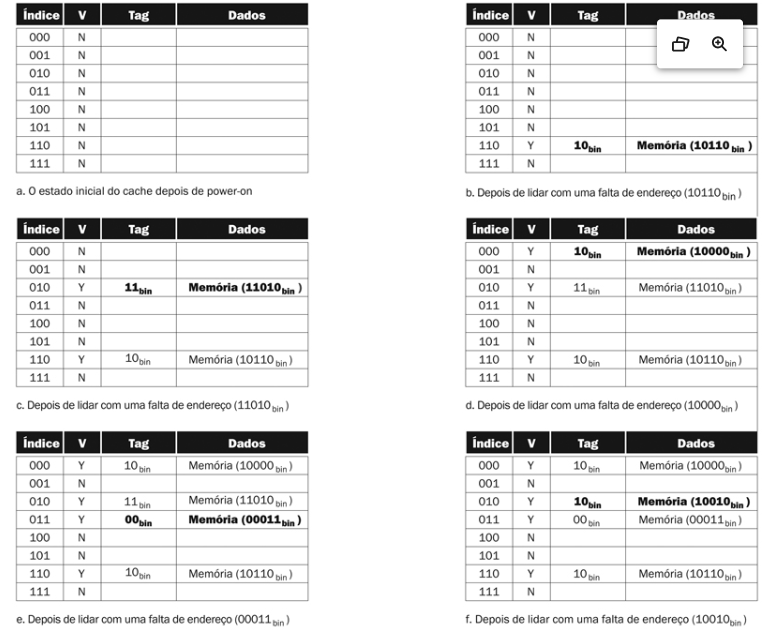
\includegraphics[width=0.8\textwidth]{figuras/localidade_temporal.png}
    \caption{Exemplo de localidade temporal (estados de uma cache)}
    \label{fig:localidade_temporal}
    \fonte{Elaborado pelos autores (2026).}
\end{figure}

\subsection{Localidade espacial}
Blocos maiores exploram a localidade espacial para diminuir as taxas de falhas. Aumentar o tamanho de bloco normalmente diminui a taxa de falhas. A taxa de falhas pode subir posteriormente se o tamanho de bloco se tornar uma fração significativa do tamanho de cache, uma vez que o número de blocos que pode ser armazenado na cache se tornará pequeno e haverá uma grande competição entre esses blocos. Explicando de outra forma: a localidade espacial entre as palavras em um bloco diminui com um bloco muito grande; por conseguinte, os benefícios na taxa de falhas se tornam menores \cite{patterson2017}.

\begin{figure}[H]
    \centering
    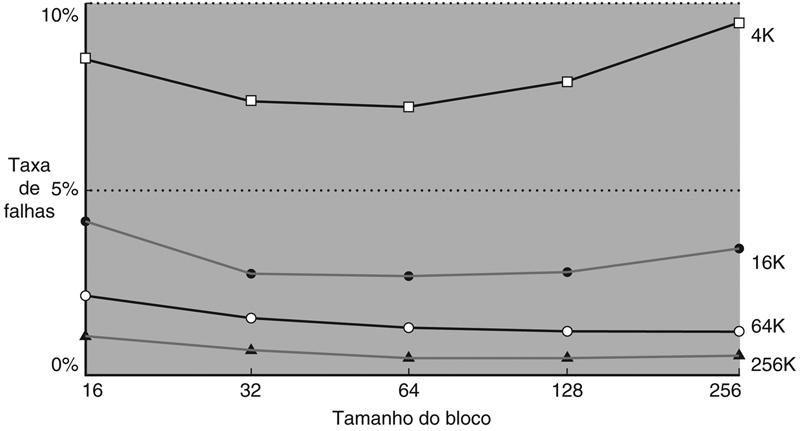
\includegraphics[width=0.7\textwidth]{figuras/localidade_tamanho_bloco.png}
    \caption{Impacto do tamanho do bloco na taxa de falhas}
    \label{fig:localidade_tamanho}
    \fonte{Elaborado pelos autores (2026).}
\end{figure}

\section{Mapeamento}
\subsection{Mapeamento direto}
A maneira mais simples de atribuir um local na cache para cada palavra da memória é atribuir um local na cache baseado no endereço da palavra na memória. Essa estrutura de cache é chamada de mapeamento direto, já que cada local da memória é mapeado diretamente para um local exato na cache.

(Endereço de bloco) módulo (Número de blocos na cache)

Se o número de entradas na cache for uma potência de dois, então, o módulo pode ser calculado simplesmente usando os \(\log_2\) bits menos significativos do endereço \cite{patterson2017}.

\begin{figure}[H]
    \centering
    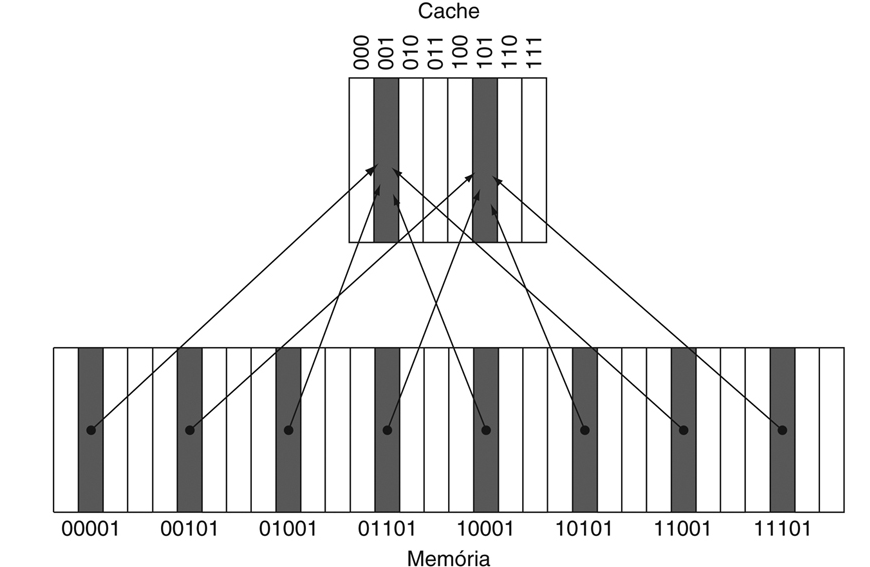
\includegraphics[width=0.8\textwidth]{figuras/mapeamento_direto.png}
    \caption{Exemplo prático de mapeamento direto na memória}
    \label{fig:mapeamento_direto}
    \fonte{Elaborado pelos autores (2026).}
\end{figure}

Como há oito palavras na cache, um endereço X é mapeado para a palavra de cache X, módulo 8. Ou seja, os \(\log_2(8) = 3\) bits menos significativos são usados como o índice da cache. Assim, os endereços \(00001_{bin}\), \(01001_{bin}\), \(10001_{bin}\) e \(11001_{bin}\) são todos mapeados para a entrada \(001_{bin}\) da cache, enquanto os endereços \(00101_{bin}\), \(01101_{bin}\), \(10101_{bin}\) e \(11101_{bin}\) são todos mapeados para a entrada \(101_{bin}\) da cache.

\subsection{Mapeamento totalmente associativo}
Até agora, quando colocamos um bloco na cache, usamos um esquema de posicionamento simples: um bloco só pode entrar exatamente em um local na cache. Como já dissemos, esse esquema é chamado de mapeamento direto porque qualquer endereço de bloco na memória é diretamente mapeado para um único local, no nível superior da hierarquia. Existe, na verdade, toda uma faixa de esquemas para posicionamento de blocos. Em um extremo está o mapeamento direto, em que um bloco só pode ser posicionado exatamente em um local.

No outro extremo está um esquema em que um bloco pode ser posicionado em qualquer local na cache. Para encontrar um determinado bloco em uma cache totalmente associativa, todas as entradas da cache precisam ser pesquisadas. Para tornar a pesquisa possível, ela é feita em paralelo com um comparador associado a cada entrada da cache. Esses comparadores aumentam muito o custo do hardware \cite{patterson2017}.

\subsection{Mapeamento associativo por conjunto}
A faixa intermediária de projetos entre a cache diretamente mapeada e a cache totalmente associativa é chamada de associativa por conjunto. Em uma cache associativa por conjunto, existe um número fixo de locais (pelo menos dois) onde cada bloco pode ser colocado. Um bloco é diretamente mapeado para um conjunto e, então, uma correspondência é pesquisada em todos os blocos no conjunto \cite{patterson2017}.

\begin{figure}[H]
    \centering
    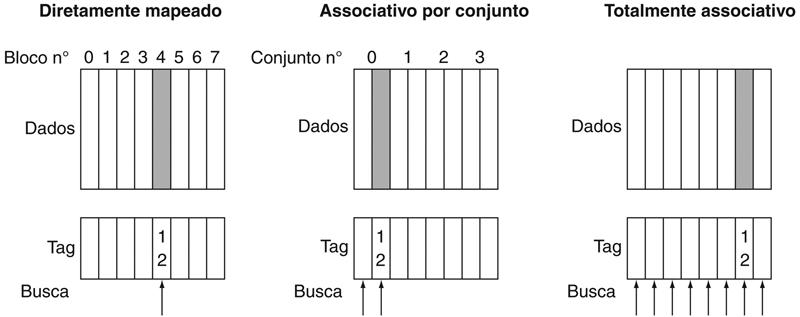
\includegraphics[width=0.9\textwidth]{figuras/tipos_mapeamento.png}
    \caption{Comparação lado a lado: mapeamento direto, associativo e totalmente associativo}
    \label{fig:tipos_mapeamento}
    \fonte{Elaborado pelos autores (2026).}
\end{figure}

\section{Políticas de escrita}
\subsection{Write-through}
A maneira mais simples de manter consistentes a memória principal e a cache é sempre escrever os dados na memória e na cache. Essas escritas levarão muito tempo, talvez mais de 100 ciclos de \textit{clock}. Uma solução é usar um \textit{buffer} de escrita \cite{hennessy2017}.

Com um esquema de \textit{write-through}, toda escrita faz com que os dados sejam escritos na memória principal. Essas escritas levarão muito tempo, talvez mais de 100 ciclos de \textit{clock} de processador, e tornariam o processador consideravelmente mais lento.

Uma solução para esse problema é usar um \textit{buffer} de escrita (ou \textit{write buffer}), que armazena os dados enquanto estão esperando para serem escritos na memória. Após escrever os dados na cache e no \textit{buffer} de dados, o processador pode continuar a execução. Quando uma escrita na memória principal é concluída, a entrada no \textit{buffer} de escrita é liberada.

Se o \textit{buffer} de escrita estiver cheio quando o processador atingir uma escrita, o processador precisará sofrer \textit{stall} até que haja uma posição vazia no \textit{buffer} de escrita. Para reduzir a ocorrência desses \textit{stalls}, os processadores normalmente aumentam a profundidade do \textit{buffer} de escrita para além de uma única entrada.

Considere uma falha em uma cache \textit{write-through}. A estratégia mais comum é alocar um bloco na cache, chamado alocar na escrita. O bloco é apanhado da memória e depois a parte apropriada do bloco é sobrescrita. Uma estratégia alternativa é atualizar a parte do bloco na memória, mas não colocá-la em cache, o que se chama não alocar na escrita. A motivação é que, às vezes, os programas escrevem blocos de dados, como quando o sistema operacional zera uma página de memória. Nesses casos, a busca associada com a falha de escrita inicial pode ser desnecessária.

\subsection{Write-back}
A alternativa é o esquema \textit{write-back}, no qual, quando ocorre uma escrita, o novo valor é escrito apenas no bloco da cache. O bloco modificado é escrito no nível inferior da hierarquia quando ele é substituído. Pode melhorar o desempenho, mas é mais complexo de implementar \cite{hennessy2017}.

Os esquemas \textit{write-back} podem melhorar o desempenho, especialmente quando os processadores podem gerar escritas tão rápido ou mais rápido do que as escritas podem ser tratadas pela memória principal; entretanto, um esquema \textit{write-back} é mais complexo de implementar do que um esquema \textit{write-through}.

Implementar \textit{stores} de modo realmente eficaz em uma cache que usa uma estratégia \textit{write-back} é mais complexo do que em uma cache \textit{write-through}. Em uma cache \textit{write-back}, precisamos escrever o bloco novamente na memória se os dados na cache estiverem modificados e tivermos uma falha de cache.

Em uma cache \textit{write-back}, como não podemos substituir o bloco, os \textit{stores} ou exigem dois ciclos (um ciclo para verificar um acerto seguido de um ciclo para efetivamente realizar a escrita) ou exigem um \textit{buffer} de escrita para conter esses dados na prática, permitindo que a \textit{store} leve apenas um ciclo por meio de um \textit{pipeline} de memória.

Muitas caches \textit{write-back} também incluem \textit{buffers} de escrita usados para reduzir a penalidade de falha quando uma falha substitui um bloco modificado. Em casos como esse, o bloco modificado é movido para um \textit{buffer write-back} associado com a cache enquanto o bloco requisitado é lido da memória. Depois, o \textit{buffer write-back} é escrito novamente na memória.

\section{Taxa de acerto e penalidade de falha}
Essa técnica é baseada na observação de que o processador normalmente precisa de apenas uma palavra do bloco de cada vez. Essa estratégia é a da impaciência: não espere até que o bloco inteiro seja carregado para então enviar a palavra solicitada e reiniciar o processador. Aqui estão duas estratégias específicas:
\begin{itemize}
    \item \textbf{Palavra crítica primeiro:} Solicite primeiro a palavra que falta e envie-a para o processador assim que ela chegar; deixe o processador continuar a execução enquanto preenche o restante das palavras no bloco.
    \item \textbf{Reinício antecipado:} Busque as palavras na ordem normal, mas, assim que a palavra solicitada chegar, envie-a para o processador e deixe que ele continue a execução.
\end{itemize}

Geralmente, essas técnicas só beneficiam projetos com grandes blocos de cache, pois o benefício é baixo, a menos que os blocos sejam grandes. Observe que, normalmente, as caches continuam a satisfazer os acessos a outros blocos enquanto o restante do bloco está sendo preenchido.

Entretanto, dada a proximidade espacial, existe boa chance de que a próxima referência seja para o restante do bloco. Assim como as caches sem bloqueio, a penalidade de falta não é simples de calcular. Quando existe uma segunda solicitação da palavra crítica primeiro, a penalidade de falta efetiva é o tempo não sobreposto da referência até que a segunda parte chegue. Os benefícios da palavra crítica primeiro e de reinício antecipado dependem do tamanho do bloco e da probabilidade de outro acesso à parte do bloco que ainda não foi acessada.

\section{Desafios comuns}
\subsection{Cache thrashing}
A função da memória cache é agilizar a execução de programas, armazenando cópias de blocos de dados da memória principal em uma memória cache mais rápida, embora de menor capacidade. O gráfico na Figura \ref{fig:cache_thrashing} ilustra a taxa de falhas (\textit{miss ratio}) de uma memória cache em função do seu tamanho e associatividade. Quanto menor for o valor da taxa de falhas, melhor será o desempenho da cache. As falhas encontradas em uma memória cache podem ser classificadas em três categorias: falhas compulsórias, por capacidade ou por conflito (também chamadas de 3 Cs) \cite{hennessy2017}.

\begin{itemize}
    \item \textbf{Falhas compulsórias:} São falhas que ocorrem sempre no primeiro acesso a um bloco, já que o bloco nunca foi armazenado na memória cache.
    \item \textbf{Falhas devido à capacidade:} São falhas que ocorrem quando a cache não consegue armazenar todos os blocos necessários à execução de um programa, por não ter capacidade suficiente.
    \item \textbf{Falhas por conflitos ou colisão:} São falhas que ocorrem quando diversos blocos competem pela mesma posição (conjunto) na memória cache. Esse tipo de falha não ocorre em caches totalmente associativas, pois neste caso um bloco pode ser armazenado em qualquer linha da memória cache.
\end{itemize}

\begin{figure}[H]
    \centering
    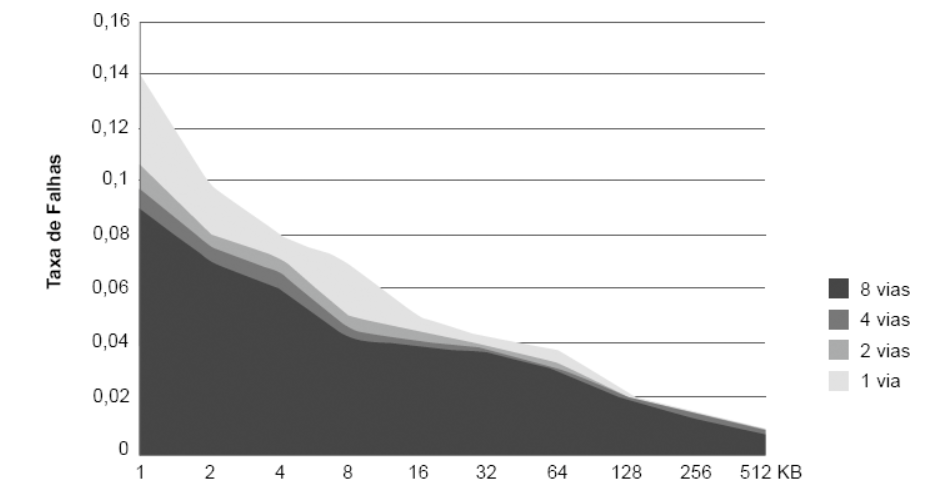
\includegraphics[width=0.8\textwidth]{figuras/localidade_espacial.png}
    \caption{Impacto da associatividade na taxa de falhas}
    \label{fig:cache_thrashing}
    \fonte{Elaborado pelos autores (2026).}
\end{figure}

\subsection{Coerência de cache em múltiplos núcleos}
Nos processadores modernos, com mais de um núcleo, é comum a existência de um terceiro nível de cache (L3), compartilhada por todos os núcleos. O tempo de acesso com acerto a essa cache é da ordem de algumas dezenas de ciclos de relógio. O uso de caches multiníveis é um recurso comum nos modernos processadores, mas que pode resultar na diminuição da taxa de acerto nos níveis mais próximos ao processador, pelo uso de caches com capacidade menor nesses níveis para acompanhar as velocidades crescentes de relógio dos processadores. A arquitetura e o desempenho final de uma memória cache devem ser adequadamente avaliados por meio de simulações, antes da sua implementação física no processador \cite{silva2024}.

\begin{figure}[H]
    \centering
    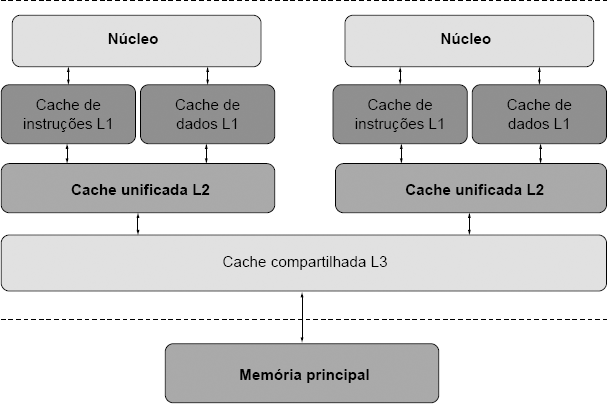
\includegraphics[width=0.8\textwidth]{figuras/hierarquia.png}
    \caption{Caches multiníveis}
    \label{fig:caches_multiniveis}
    \fonte{Elaborado pelos autores (2026).}
\end{figure}

\subsection{Falso compartilhamento}
No início dos tempos a memória cache está vazia, ou seja, não possui nenhuma informação armazenada e todas as suas linhas estão marcadas como inválidas. As instruções e dados vão sendo então gradativamente copiados dos níveis inferiores, como a memória principal e secundária, para a memória cache, à medida que são utilizados pelo processador. Na realidade, o processador inicia a busca das instruções ou dos dados na suposição de que estejam armazenados na memória cache. Se forem encontrados na memória cache (houve um acerto), a informação desejada é transferida para o processador. Mas se os dados ou a instrução não estiverem na memória cache (houve uma falha), então o processador aguarda, enquanto a instrução/dados desejados são copiados para a memória cache e depois transferidos para o processador.

Durante a busca da informação que está faltando na cache, em vez de trazer somente a instrução ou dados solicitados pelo processador, um bloco inteiro é copiado da memória principal e armazenado em uma linha da cache, que então é marcada como válida. O objetivo é minimizar a taxa de falhas nos próximos acessos, seguindo o princípio da localidade espacial. O tamanho de um bloco é um parâmetro de projeto nas memórias caches, tamanhos usuais são 32, 64 e 128 bytes. Note que um bloco trazido da memória principal recebe o nome de linha quando armazenado na memória cache, sendo, portanto, de mesmo tamanho \cite{silva2024}.

\section{Técnicas de otimização}
Essas otimizações aumentam a largura de banda da cache seja pelo \textit{pipelining} do acesso à cache ou pela ampliação da cache com múltiplos bancos, permitindo múltiplos acessos por ciclo de \textit{clock}; essas otimizações estão associadas às abordagens \textit{superpipelined} e superescalar para aumentar o \textit{throughput} de instrução. Elas visam principalmente a cache L1, onde a largura de banda de acesso restringe o \textit{throughput} de instrução.

O \textit{pipelining} L1 permite um ciclo de \textit{clock} mais alto, ao custo de uma maior latência. O \textit{pipelining} da cache de instruções efetivamente aumenta o número de estágios do \textit{pipeline}, levando a uma penalidade maior nos desvios mal previstos. De modo correspondente, o \textit{pipelining} da cache de dados leva a mais ciclos de \textit{clock} entre a emissão do \textit{load} e o uso dos dados.

Para lidar com múltiplos acessos à cache de dados por \textit{clock}, podemos dividir a cache em bancos independentes, cada um suportando um acesso independente. Os bancos foram originalmente usados para melhorar o desempenho da memória principal e agora são usados dentro de chips DRAM modernos, bem como com caches. O Intel Core i7 contém quatro bancos na cache L1 (para admitir até 2 acessos de memória por \textit{clock}) \cite{hennessy2019}.

Uma cache sem bloqueio ou cache sem travamento aumenta os benefícios em potencial de tal esquema, permitindo que a cache de dados continue a fornecer acertos de cache durante uma falta. Essa otimização de ``acerto sob falta'' reduz a penalidade de falta efetiva, sendo útil durante uma falta, em vez de ignorar as solicitações do processador. Uma opção sutil e complexa é que a cache pode reduzir ainda mais a penalidade de falta efetiva se puder sobrepor múltiplas faltas: uma otimização ``acerto sob múltiplas faltas'' ou ``falta sob falta''. A segunda opção só será benéfica se o sistema de memória puder atender a múltiplas faltas; a maior parte dos processadores de alto desempenho (como os processadores Intel Core) geralmente suporta ambos, enquanto muitos dos processadores de baixo nível oferecem somente suporte limitado sem bloqueio na cache L2 \cite{hennessy2019}.

Até aqui, nossas técnicas têm exigido a mudança do hardware. Essa próxima técnica reduz as taxas de falta sem quaisquer mudanças no hardware. Essa redução mágica vem do software otimizado a solução favorita do projetista de hardware! A diferença de desempenho cada vez maior entre os processadores e a memória principal tem inspirado os projetistas de compiladores a investigar a hierarquia de memória para ver se as otimizações em tempo de compilação podem melhorar o desempenho. Mais uma vez, a pesquisa está dividida entre as melhorias nas faltas de instrução e as melhorias nas faltas de dados. As otimizações apresentadas a seguir são encontradas em muitos compiladores modernos.

Em vez de operar sobre linhas ou colunas inteiras de um \textit{array}, os algoritmos bloqueados operam sobre submatrizes ou blocos. O objetivo é maximizar os acessos aos dados carregados na cache antes que eles sejam substituídos \cite{hennessy2019}.

As caches sem bloqueio reduzem efetivamente a penalidade de falta, sobrepondo a execução com o acesso à memória. Outra técnica é fazer a pré-busca (\textit{prefetch}) dos itens antes que o processador os solicite. Tanto as instruções quanto os dados podem ter sua busca antecipada, seja diretamente nas caches, seja diretamente em um buffer externo, que pode ser acessado mais rapidamente do que a memória principal.

Frequentemente, a pré-busca de instrução é feita no hardware fora da cache. Em geral, o processador apanha dois blocos em uma falta: o bloco solicitado e o próximo bloco consecutivo. O bloco solicitado é colocado na cache de instruções, e o bloco cuja busca foi antecipada é colocado no buffer do fluxo de instruções. Se o bloco solicitado estiver presente no buffer do fluxo de instruções, a solicitação de cache original será cancelada, o bloco será lido do buffer de fluxo e a próxima solicitação de pré-busca será emitida \cite{hennessy2019}.
\chapter{Mapeamento e diagrama arquitetural}
\label{cap:diagramas}

\section{Hierarquia de memória}
O sistema de memória de dados modelado com base no Intel i7 consiste em uma cache L1 de 32 KiB, com latência de acesso de quatro ciclos. A cache L2 (compartilhada com instruções) é de 256 KiB, com uma latência de acesso de 10 ciclos de \textit{clock}. A cache L3 tem 2 MiB e uma latência de acesso de 36 ciclos. Todas as caches são associativas por conjunto de oito vias e têm tamanho de bloco de 64 bytes. Permitir um acerto sob falta reduz a penalidade de falta em 9\% para os \textit{benchmarks} inteiros e de 12,5\% para os de ponto flutuante. Permitir um segundo acerto melhora esses resultados para 10\% e 16\%, e permitir 64 resulta em pouca melhoria adicional \cite{hennessy2019}.

\section{Divisão do endereço}
As caches possuem uma \textit{tag} de endereço em cada \textit{frame} de bloco, que indica o endereço do bloco. A \textit{tag} de cada bloco da cache que poderia conter a informação desejada é verificada, para saber se corresponde ao endereço de bloco do processador. Em geral, todas as \textit{tags} possíveis são pesquisadas em paralelo, pois a velocidade é crítica.

É preciso haver um meio de saber que um bloco de cache não tem informação válida. O procedimento mais comum é acrescentar um bit de validade à \textit{tag} para dizer se essa entrada contém ou não um endereço válido. Se o bit não for definido, não poderá haver uma combinação nesse endereço.

Antes de passar à próxima pergunta, vamos explorar o relacionamento de um endereço do processador com a cache. A primeira divisão ocorre entre o endereço de bloco e o \textit{offset} de bloco. O endereço do \textit{frame} de bloco pode ser dividido ainda mais, em campo de \textit{tag} e campo de índice. O campo de \textit{offset} de bloco seleciona os dados desejados do bloco, o campo de índice seleciona o conjunto e o campo de \textit{tag} é comparado com ele para ver se há um acerto. Embora a comparação pudesse ser feita sobre mais de um endereço do que a \textit{tag}, isso não é necessário, devido ao seguinte:
\begin{itemize}
    \item O \textit{offset} não deve ser usado na comparação, pois ou o bloco inteiro está presente ou não, e por isso todos os \textit{offsets} de bloco resultam em uma combinação por definição.
    \item A verificação do índice é redundante, pois foi usada para selecionar o conjunto a ser verificado. Um endereço armazenado no conjunto 0, por exemplo, precisa ter 0 no campo de índice ou não poderia ser armazenado no conjunto 0; o conjunto 1 precisa ter um valor de índice igual a 1, e assim por diante. Essa otimização economiza hardware e energia, reduzindo o tamanho da memória para a \textit{tag} de cache.
\end{itemize}

\begin{table}[H]
    \centering
    \begin{tabular}{|l|l|l|}
        \hline
        \multicolumn{2}{|c|}{Endereço de bloco} & \multirow{2}{*}{Offset de bloco} \\ \cline{1-2}
        Tag & Índice & \\ \hline
    \end{tabular}
    \caption{As três partes de um endereço em uma cache associativa em conjunto ou com mapeamento direto.}
    \label{tab:endereco}
    \fonte{Elaborado pelos autores (2026).}
\end{table}

A \textit{tag} é usada para verificar todos os blocos no conjunto, e o índice é usado para selecionar o conjunto. O \textit{offset} de bloco é o endereço dos dados desejados dentro do bloco. As caches totalmente associativas não possuem campo de índice.

Se o tamanho total da cache for mantido igual, o aumento da associatividade aumentará o número de blocos por conjunto, diminuindo assim o tamanho do índice e aumentando o tamanho da \textit{tag}. Ou seja, o limite de índice de \textit{tag} se move para a direita aumentando-se a associatividade, com a extremidade das caches totalmente associativas não possuindo campo de índice \cite{hennessy2019}.

\section{Esquema de cada mapeamento}
Podemos pensar em cada estratégia de posicionamento de bloco como uma variação da associatividade por conjunto. Uma cache diretamente mapeada é simplesmente uma cache associativa por conjunto de uma via: cada entrada de cache contém um bloco, e cada conjunto possui um elemento. Uma cache totalmente associativa com m entradas é simplesmente uma cache associativa por conjunto de m vias; ele tem um conjunto com m blocos, e uma entrada pode residir em qualquer bloco dentro desse conjunto. O tamanho total da cache em blocos é igual ao número de conjuntos multiplicado pela associatividade. Portanto, para uma cache de tamanho fixo, aumentar a associatividade diminui o número de conjuntos enquanto aumenta o número de elementos por conjunto \cite{hennessy2017}.

\begin{figure}[H]
    \centering
    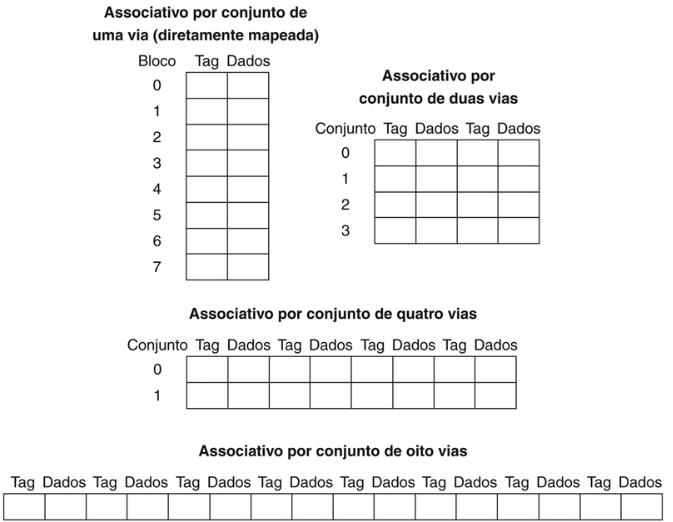
\includegraphics[width=0.9\textwidth]{figuras/endereco.png}
    \caption{Esquemas de mapeamento de cache}
    \label{fig:mapeamentos}
    \fonte{Elaborado pelos autores (2026).}
\end{figure}

\section{Fluxo de acesso à cache}
A \textit{tag} da cache é comparada com a parte superior do endereço para determinar se a entrada na cache corresponde ao endereço requisitado. Como a cache tem \(2^{10}\) (ou 1024) palavras e um tamanho de bloco de 1 palavra, 10 bits são usados para indexar a cache, deixando \(32 - 10 - 2 = 20\) bits para serem comparados com a \textit{tag}. Se a \textit{tag} e os 20 bits superiores do endereço forem iguais e o bit de validade estiver ligado, então, a requisição é um acerto na cache e a palavra é fornecida para o processador. Caso contrário, ocorre uma falha.

A unidade de controle precisa detectar uma falha de cache e processá-la buscando os dados requisitados da memória (ou, como veremos, de uma cache de nível inferior). Se a cache reportar um acerto, o computador continua usando os dados como se nada tivesse acontecido \cite{patterson2017}.

\section{Cache da máquina usada na PoC}
\label{sec:cache-poc}
A máquina utilizada para os testes da PoC possui um processador Intel Core i5-12500H (12ª geração) e sistema operacional Fedora Linux. De acordo com o comando \texttt{lscpu}, a hierarquia de cache é composta por 448 KiB de cache L1 de dados (L1d), 640 KiB de cache L1 de instruções (L1i), 9 MiB de cache L2 e 18 MiB de cache L3 compartilhada.
\chapter{Metodologia e desenvolvimento}
\label{cap:metodologia}

A metodologia utilizada neste trabalho consiste no desenvolvimento de uma Prova de Conceito (PoC) com o objetivo de analisar e comparar o desempenho de dois métodos de acesso aos elementos de uma matriz bidimensional: o percurso linha por linha e o percurso coluna por coluna. A proposta busca demonstrar como a organização dos dados na memória e a forma como eles são acessados podem influenciar diretamente o desempenho de um programa.

Para realizar essa comparação, foram implementados algoritmos em linguagem C, utilizando uma matriz com dimensões previamente definidas. Os dois métodos executam operações sobre os mesmos elementos, porém seguindo ordens diferentes de acesso à memória. Dessa forma, é possível observar diferenças no tempo de execução e compreender a influência da hierarquia de memória, especialmente da memória cache, no desempenho computacional.

\section{Ambiente de teste}
Os testes foram realizados em um ambiente computacional com o objetivo de garantir condições semelhantes para a execução dos dois algoritmos. Para isso, foram utilizados o mesmo computador, sistema operacional, compilador e configurações de execução. A linguagem C foi escolhida por permitir maior controle sobre o acesso à memória.

\section{Ferramentas de medição}
Para avaliar o desempenho dos algoritmos, foram utilizadas ferramentas de medição de tempo de execução disponíveis na linguagem C e no ambiente de desenvolvimento.
A medição do tempo permite identificar quanto tempo cada algoritmo leva para percorrer todos os elementos da matriz. Essa informação é importante para compreender como diferentes estratégias de acesso aos dados podem produzir resultados distintos, mesmo quando realizam a mesma quantidade de operações.
Além disso, podem ser utilizadas ferramentas de monitoramento de desempenho do sistema para observar aspectos como utilização do processador e comportamento da memória cache. Essas informações complementam os resultados obtidos pela medição do tempo de execução.
É importante realizar várias execuções de cada algoritmo e calcular uma média dos resultados, reduzindo a influência de possíveis variações ocasionais do sistema.

\section{Algoritmos implementados}
Foram desenvolvidos dois algoritmos com a finalidade de comparar diferentes formas de percorrer uma matriz bidimensional. Na linguagem C, as matrizes são armazenadas na memória seguindo uma organização denominada \textit{row-major order}.

\subsection{Percurso linha por linha}
O primeiro algoritmo realiza o acesso aos elementos da matriz percorrendo inicialmente todas as colunas de uma linha antes de avançar para a próxima linha. Como os elementos de uma mesma linha estão armazenados em posições consecutivas da memória, o processador consegue aproveitar melhor os dados carregados previamente para a memória cache.

\clearpage

\lstinputlisting[style=cstyle, caption={Código em C para o percurso linha por linha}, label={lst:linha}]{poc/percurso_linha.c}

\subsection{Percurso coluna por coluna}
O segundo algoritmo percorre uma coluna inteira antes de avançar para a próxima. Embora todos os elementos sejam acessados, essa estratégia não acompanha a ordem em que os dados estão organizados na memória, apresentando menor aproveitamento da memória cache.

\clearpage

\lstinputlisting[style=cstyle, caption={Código em C para o percurso coluna por coluna}, label={lst:coluna}]{poc/percurso_coluna.c}

\section{Passo a passo da PoC}
\begin{enumerate}
    \item Criação e inicialização da matriz bidimensional.
    \item Implementação do percurso linha por linha (dois laços de repetição).
    \item Desenvolvimento do percurso coluna por coluna (invertendo a ordem dos laços).
    \item Medição do tempo de execução de cada algoritmo.
    \item Análise dos dados considerando a organização da memória.
\end{enumerate}

\section{Métricas coletadas}
As principais métricas consideradas foram o tempo de execução e a diferença de desempenho entre os dois métodos. Também foram considerados indicadores como a quantidade de acertos (\textit{cache hits}) e falhas (\textit{cache misses}).

\section{Limitações do método}
A metodologia apresenta limitações relacionadas ao hardware utilizado, fatores como processos em segundo plano, temperatura do processador e otimizações do compilador. O tamanho da matriz também influencia, pois se os dados couberem completamente na cache, a diferença entre os algoritmos será reduzida.
\chapter{Discussão dos resultados}
\label{cap:discussao}

A discussão dos resultados tem como objetivo interpretar os dados obtidos durante a execução dos algoritmos e relacioná-los aos conceitos de arquitetura de computadores e organização da memória. A comparação entre os percursos linha por linha e coluna por coluna permite observar que a ordem de acesso aos dados influencia diretamente o desempenho de aplicações que trabalham com matrizes.

\begin{table}[H]
    \centering
    \caption{Comparação entre os dois padrões de acesso à memória}
    \label{tab:comparacao}
    \begin{tabular}{lcc}
        \toprule
        \textbf{Métrica} & \textbf{Linha por linha} & \textbf{Coluna por coluna} \\
        \midrule
        Tempo de execução (s) & 0,006974 & 0,010819 \\
        Soma calculada & 4194304 & 4194304 \\
        L1 cache misses & 61.204 & 5.444.797 \\
        LLC cache misses & 126.655 & 320.348 \\
        \bottomrule
    \end{tabular}
    \fonte{Elaborado pelos autores com dados do \texttt{perf stat} (2026).}
\end{table}

\section{Análise da comparação}
Os resultados demonstram uma diferença significativa de desempenho entre os dois métodos. O percurso linha por linha executou a tarefa em aproximadamente 0,006 segundos, enquanto o percurso coluna por coluna levou cerca de 0,011 segundos. Isso representa um tempo cerca de 55\% maior para o algoritmo que percorre as colunas.

\section{Do código em C ao hardware}
A execução de um programa em C envolve uma interação direta entre o software e os componentes físicos. Quando um programa acessa um elemento de uma matriz, o processador precisa obter o dado na hierarquia de memória. Na linguagem C, a organização \textit{row-major} faz com que o percurso linha por linha aproveite melhor os dados já carregados na cache.

No percurso linha por linha, o processador acessa posições consecutivas da memória, favorecendo o aproveitamento dos blocos de dados. No percurso coluna por coluna, os acessos ocorrem em posições mais distantes, provocando mais falhas de cache. Dessa forma, mesmo com a mesma complexidade assintótica (\(O(n \times m)\)), os desempenhos práticos são diferentes.

\section{Limitações do método}
Os resultados apresentados possuem limitações, como a dependência das configurações do compilador e as características do processador. Variações nos tempos de execução podem ocorrer devido ao sistema operacional e à execução de outros processos.

\section{Limitações físicas}
As limitações físicas estão relacionadas às características dos componentes de hardware. A memória cache possui capacidade limitada, enquanto a memória RAM apresenta maior latência. A largura de banda da memória e o tamanho dos blocos transferidos também influenciam o desempenho.

\section{Impacto no desenvolvimento de software de alto desempenho}
O estudo demonstra que a organização dos dados e a escolha dos padrões de acesso à memória são fundamentais. A utilização adequada da memória cache pode reduzir o tempo de execução e melhorar a eficiência dos recursos computacionais, especialmente em aplicações científicas, processamento de imagens e inteligência artificial.
\chapter{Conclusão}
\label{cap:conclusao}

O desenvolvimento deste trabalho permitiu analisar a influência dos padrões de acesso à memória no desempenho de programas desenvolvidos em linguagem C. A partir da implementação dos algoritmos de percurso linha por linha e coluna por coluna, foi possível estudar como a organização dos dados na memória interfere na execução de operações sobre matrizes bidimensionais. Os conceitos estudados demonstram que pequenas alterações na estrutura de um programa podem produzir diferenças significativas de desempenho, especialmente quando são utilizados grandes conjuntos de dados.

\section{Síntese do aprendizado}
Durante o desenvolvimento da atividade, foi possível compreender a importância da hierarquia de memória e sua influência na execução de programas. O estudo demonstrou que a memória cache desempenha um papel fundamental na redução do tempo de acesso aos dados, permitindo que o processador trabalhe de maneira mais eficiente.

Também foi possível compreender que a linguagem C utiliza uma organização de memória na qual os elementos de uma mesma linha de uma matriz são armazenados de forma sequencial. Dessa maneira, o percurso linha por linha tende a proporcionar melhor aproveitamento da memória cache em comparação ao percurso coluna por coluna.

\section{Lições aprendidas}
Uma das principais lições aprendidas foi que a eficiência de um algoritmo não depende apenas de sua complexidade teórica. Embora os dois métodos implementados apresentem a mesma complexidade assintótica, o comportamento durante a execução pode ser diferente devido à organização dos dados na memória.

Outro aprendizado importante foi a necessidade de realizar testes práticos para avaliar o desempenho de um programa. A análise teórica permite formular hipóteses, mas as medições são fundamentais para verificar como o código se comporta em um ambiente real.

\section{Implicações práticas}
Os conhecimentos adquiridos durante o trabalho podem ser aplicados em diferentes áreas da computação, principalmente em programas que realizam operações com grandes volumes de dados. Em aplicações de processamento de imagens, cálculos científicos, inteligência artificial e simulações computacionais, a organização dos dados e a forma de acesso à memória podem influenciar diretamente o tempo necessário para concluir uma tarefa. Assim, utilizar padrões de acesso que favoreçam a localidade espacial pode contribuir para melhorar o desempenho das aplicações.

Conclui-se que o desenvolvimento de software eficiente exige não apenas conhecimentos de programação, mas também compreensão sobre o funcionamento do hardware. A análise realizada evidencia a importância de considerar a interação entre código, processador e memória durante o desenvolvimento de soluções computacionais.

% --- Pós-textuais ---
\postextual
% O nocite abaixo serve para incluir na lista de referências os livros que não foram citados diretamente no texto, mas que fazem parte da fundamentação
\nocite{monteiro2007,weber2012,valgrind,intel2024,stallings2017,tanenbaum2013}
\bibliography{referencias}

\end{document}